\chapter{Methods}


\section{Design}
%-------------------------------------------%

Our game agent will use the SerpentAI API to retrieve the frame buffer from the game's runtime. This buffer will then be passed to our TensorFlow neural network via Keras. The neural network will interpret the frame buffer and then produce an output consisting of up to two simultaneous button presses, which will get passed all the way back along the chain to the game runtime. Through all of this, SerpentAI will be making frequent use of a Redis database as well as modules provided by Anaconda. Also, TensorFlow will utilize the GPU for its computations using the CUDA toolkit.

\begin{figure}
	\caption{Data flow within our software stack}
	\centering
		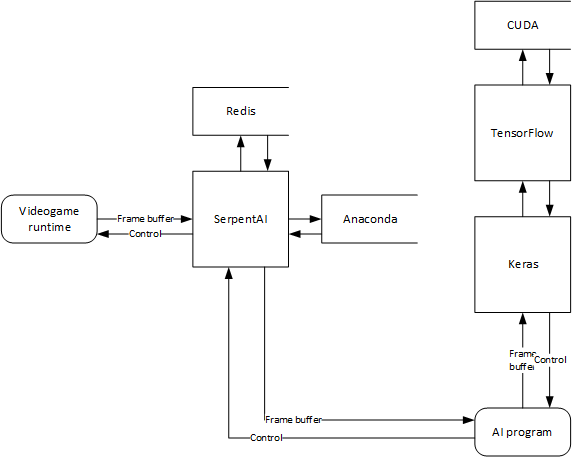
\includegraphics[scale = 0.75]{dataflow.png} \\
\end{figure}

%-------------------------------------------%

\section{Frameworks}
%-------------------------------------------%

Our project uses a software stack comprised of the following modules and libraries: SerpentAI, Keras, TensorFlow, and the Anaconda Distribution for Python 3. We chose to use Python 3 as our primary programming language for its flexibility, intuitive syntax, and data processing capabilities. Python is also helpfully compatible with all of the other software listed above. Furthermore, the {\it Anaconda distribution} provides us with a large assortment of Python modules, some of which {\it SerpentAI} cites as dependencies \cite{SerpentAI}. This allows us to more easily work from within a Windows environment, which in turn gives us the most straightforward and stable access to GPU computation via NVIDIA proprietary drivers. TensorFlow serves as the project's backbone by actually creating the neural network in addition to performing the necessary computations \cite{TensorFlow}, with Keras allowing us to perform rapid prototyping in TensorFlow via its abstracted API \cite{Keras}.

All experiments will take place on a pair of 64-bit Windows 10 machines with Ubuntu subsystems. There are several reasons to justify this decision. Firstly, we wanted to ensure that we would have the best possible experience when dealing with GPU computation, and NVIDIA simply has a longer and better track record for supporting Windows than it does for Linux. Secondly, we wanted to avoid the potential pitfall of our platform restricting us to a smaller library of target games. Our two top candidates were Quake and Rivals of Aether because both of these games support replays, or demos; however, of those two games, only Quake natively supports Linux, and ultimately we selected Rivals of Aether. Lastly, and with regards to using our own computers for both development and testing: we made the decision to abstain from distributed or cloud computing chiefly to save costs, but also as an aesthetic choice based in our desire to push our own hardware to its absolute limits. Despite all of the above justifications for using Windows, it remains to be said that our project cannot live without Linux. SerpentAI requires a Redis database, so in order for that to work we use an Ubuntu subsystem; this is the official recommendation from the SerpentAI developers \cite{SerpentAI}.

%-------------------------------------------%



\section{Algorithms}
%-------------------------------------------%

Our approach to creating this AI is to use a modular multi-layer recurrent neural network. One of the modules will parse the visual buffer using either scene segmentation or a autoencoder, depending on which of these techniques yields better results. The goal is to have the AI plan its actions and then learn from its guesses by using the recurrent neural network model. Furthermore, it will be able to understand more abstract qualities of the visual buffer by using its multiple layers.

The specific RNN model we use will change as we experiment. Training shall be achieved using gradient descent.

%-------------------------------------------%



\section{Features}
%-------------------------------------------%

In order to play Rivals of Aether, one must use a set of controls containing a total of nine buttons, where five are for actions such as attacking or dodging and four are for movement.

\begin{figure}
	\caption{In-game menu displaying game controls}
	\centering
	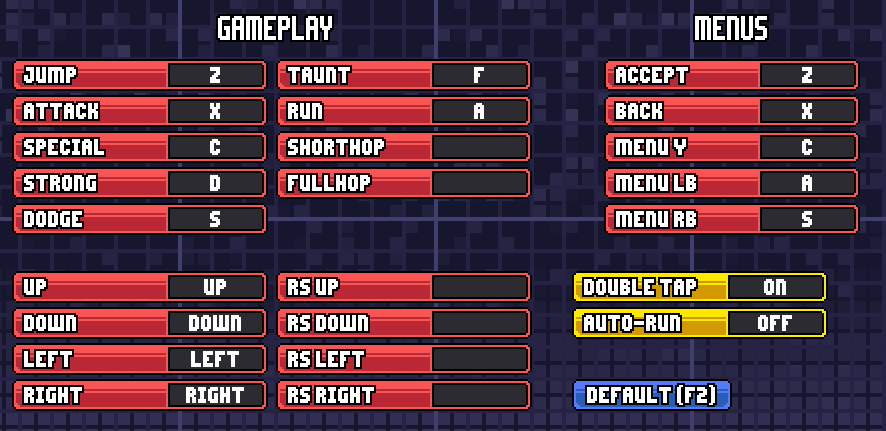
\includegraphics[scale = 0.5]{controls.png} \\
\end{figure}

These buttons can be combined for different effects. An attack will undergo significant changes depending on if the attacking character is standing, walking, running, or jumping. Furthermore, tilting the control stick during the attack will effect additional changes. Dodging in the air is different from doing so on the ground, which is different still from dodging while moving the control stick in a direction.

Due to the complex nature of the game's control scheme, at any given moment the AI will need to be able to output any combination of two simultaneous button presses, where one of the buttons is for movement and the other is for an action.

%-------------------------------------------%



\section{Test Plan}
%-------------------------------------------%

We have over 1,000 data points in the form of replay files. This dataset will be randomly distributed such that around eighty-percent goes into a training set, fifteen-percent into a testing set, and the remainder into a validation set.

A training session will run as follows. The SerpentAI agent will traverse the game's menus to initiate playback of the next replay from a shuffled copy of the training set. While the match is simulated, the agent will simultaneously read the visual buffer from the game and control input data from the replay file. For each frame, the agent will pair the input data with its corresponding visual buffer and then send this bundle to a TensorFlow neural network as labels and data, respectively. The neural network will attempt to produce a set of appropriate control inputs in response and adjust its weights  whenever its prediction are incorrect. When playback has concluded, the agent will traverse the menus once again to start a new replay, repeatedly, until it has reached its quota. The total number of training iterations will vary between experiments until it produces satisfactory results.

A properly trained neural network shall demonstrate several qualities other than a high accuracy when tested against the held back data. Firstly, it shall be able to defeat low-level in-game bots, thereby demonstrating its competence. This can be tested by placing the neural network in matches against bots of increasing difficulty, thereby enabling the assignment of numerical performance benchmarks. Secondly, it shall play in a believably-human manner. This means that it should, wherever possible, be discouraged from playing {\it inhumanly} well, getting stuck, or displaying mechanical tics. Examples of these undesirable behaviors would include, in order, executing nonstop frame-perfect moves throughout the course of an entire game, running off of the stage or standing still due to an as-of-yet unseen situation, or constantly changing direction for no reason while otherwise playing competently. Identifying all such behaviors will be difficult prior to live experiments, however.

%-------------------------------------------%



\section{Criteria and Constraints}
%-------------------------------------------%

Initial work on the neural network implementation is due to start on December 12, 2017, shortly after the conclusion of the 2017 Fall Semester. This work should be concluded by mid-March. From there, about two weeks are allocated for finalizing the design document. Overall, the schedule is intentionally tight in order to emphasize getting most of the work done in the beginning of the semester, thereby maximizing flex time and minimizing the competition between this project and other finals.

\begin{figure}
	\caption{Gantt chart}
	\centering
	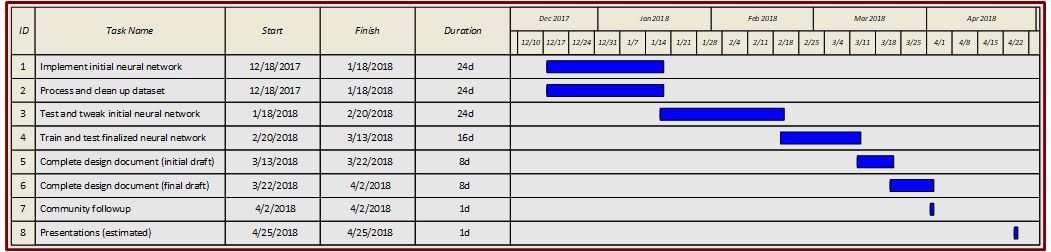
\includegraphics[scale = 0.5]{gantt.png} \\
\end{figure}

The project has other constraints in addition to its schedule. The dataset was collected from the community with the promise that each replay file we receive will be treated as private data and not, under any circumstances, be redistributed. Thus, care shall be taken to ensure that no replay files from the community are leaked. At the same time, however, these files must not be lost due to accidental deletion, disk failure, or lack of backup. To address these requirements, multiple redundant copies of the dataset are stored on our own local drives as well as via encrypted, private, cloud storage services such as Google Drive. Only the dozen or so replay files that we brought to the dataset ourselves may be stored publicly on the GitHub repository.

Our experiments will be deemed adequately successful if we can produce AI that beat the in-built bots on lowest difficulty levels. This is considered a baseline that we will attempt to surpass through improvements to the neural network and additional training.

%-------------------------------------------%
